\documentclass{standalone}
\usepackage{tikz}
\usepackage{ctex,siunitx}
\setCJKmainfont{Noto Serif CJK SC}
\usepackage{tkz-euclide}
\usepackage{amsmath}
\usetikzlibrary{patterns, calc}
\usetikzlibrary {decorations.pathmorphing, decorations.pathreplacing, decorations.shapes,}

\begin{document}
\small
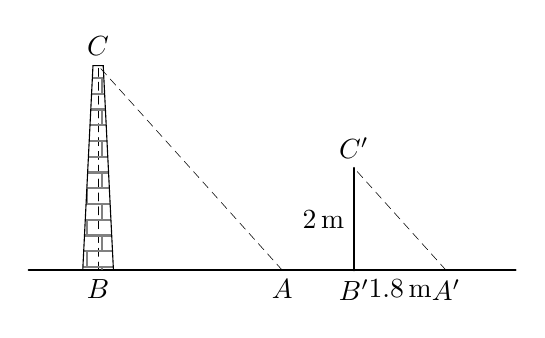
\begin{tikzpicture}[>=stealth,scale=0.65]
  \tkzSetUpPoint[fill=black]
  % \useasboundingbox(-1,-0.75)rectangle(3.7,1.4);
  \tkzDefPoints{3.6/0/A, 0/0/B, 0/4/C, 6.8/0/A', 5/0/B', 5/2/C',0.1/4/M,-0.1/4/N,-0.3/0/P,0.3/0/Q}
  \tkzDrawSegments[densely dashed](A,C B,C A',C')
  \tkzDrawSegments[thick](B',C')
  \tkzDrawLine[semithick](B,A')
  \tkzLabelPoints(A,B,A',B')
  \tkzLabelPoints[above](C,C')
  \draw[pattern=bricks,pattern color=gray](M)--(N)--(P)--(Q)--cycle;
  \node at (5.9,0)[below]{\qty{1.8}{m}};
  \node at (5,1)[left]{\qty{2}{m}};
\end{tikzpicture}
\end{document}